%
%
%%changer le format des sections, subsections pour apparaittre sans le num de chapitre
%\makeatletter
%\renewcommand{\thesection}{\@arabic\c@section}
%\makeatother
%
%%recommencer la numérotation des section à "1"
%
%%\addcontentsline{toc}{subsection}{Organisation tests CPU}
%\begin{figure}
%\centering
%\includegraphics[angle=90,scale=0.35]{images/grapheCPU.png}
%\caption{Graphe d'organisation des tests du CPU}
%\end{figure}
%
%
%%\addcontentsline{toc}{subsection}{Organisation tests HDD}
%\begin{figure}
%\centering
%\includegraphics[angle=90,scale=0.45]{images/grapheHDD.png}
%\caption{Graphe d'organisation des tests HDD}
%\end{figure}
%
%
%
%
%%\addcontentsline{toc}{subsection}{Organisation tests network}
%\begin{figure}
%\centering
%\includegraphics[angle=90,scale=0.40]{images/grapheNT.png}
%\caption{Graphe d'organisation des tests sur le network}
%\end{figure}
%
%%\addcontentsline{toc}{subsection}{Organisation du stage}
%\begin{figure}
%\centering
%\includegraphics[angle=90,scale=0.5]{images/graphe.png}
%\caption{Graphe d'organisation du stage}
%\end{figure}
%%\addcontentsline{toc}{subsection}{Organisation sonde personnelle}
%\begin{figure}
%\centering
%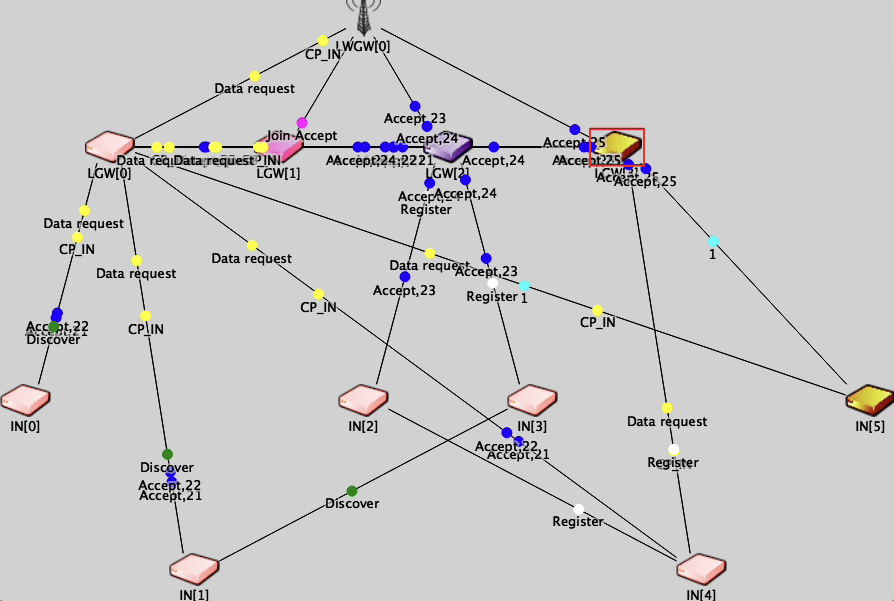
\includegraphics[scale=1]{images/fat.png}
%\caption{Graphe d'organisation de type Fat tree}
%\end{figure}

